\documentclass[11pt,a4paper,twoside]{report}
\usepackage{isabelle,isabellesym}

% further packages required for unusual symbols (see also
% isabellesym.sty), use only when needed

%\usepackage{amssymb}
  %for \<leadsto>, \<box>, \<diamond>, \<sqsupset>, \<mho>, \<Join>,
  %\<lhd>, \<lesssim>, \<greatersim>, \<lessapprox>, \<greaterapprox>,
  %\<triangleq>, \<yen>, \<lozenge>

%\usepackage{eurosym}
  %for \<euro>

%\usepackage[only,bigsqcap]{stmaryrd}
  %for \<Sqinter>

%\usepackage{eufrak}
  %for \<AA> ... \<ZZ>, \<aa> ... \<zz> (also included in amssymb)

%\usepackage{textcomp}
  %for \<onequarter>, \<onehalf>, \<threequarters>, \<degree>, \<cent>,
  %\<currency>

%\usepackage[utf8]{inputenc}
%\usepackage[T1]{fontenc}
\usepackage{amsmath}
\usepackage{array}
\usepackage{amsfonts}
\usepackage{tikz}
\usepackage[inline]{enumitem}
\usepackage{varwidth}

\usetikzlibrary{arrows}

% this should be the last package used
\usepackage{pdfsetup}

% urls in roman style, theory text in math-similar italics
\urlstyle{rm}
\isabellestyle{it}

% for uniform font size
%\renewcommand{\isastyle}{\isastyleminor}
%
\hyphenation{Isa-belle}


\begin{document}

\title{Formalizing \emph{Types and Programming Languages} in Isabelle/HOL}
\author{Martin Desharnais}

\pagenumbering{roman}
\maketitle

\begin{abstract}
We formalized, using Isabelle/HOL, some languages presented in the first two sections, namely
"Untyped Systems" and "Simple Types", of the book \emph{Types and Programming Languages} by
Benjamen~C.~Pierce. We first begin with a short tour of lambda-calculus, type theory and the
Isabelle/HOL theorem prover before attacking the formalization per se. Starting with an arithmetic
expression language offering booleans and natural numbers, we pursue, after a brief digression to
the "de Bruijn indices", to the untyped lambda-calculus. We then return to a typed variant of the
arithmetic expression language before to conclude with the simply typed lambda-calculus.
\end{abstract}

\tableofcontents

\cleardoublepage
\pagenumbering{arabic}
\pagestyle{headings}

\section{Introduction}

This bachelor thesis deals with the formalisation, in the Isabelle/HOL theorem prover, of parts of
the book \emph{Types and Programming Languages}, hereafter abbreviated \emph{TAPL}, by
Benjamen~C.~Pierce. This work concentrate on four of the languages, ranging from simple arithmetic
expressions to the fully fledged lambda-calculus, present in the first two sections, namely "Untyped
Systems" and "Simple Types".

The main motivation to have chosen this subject is the intersection of personal interest and of
opportunities provided by our intership at the chair for logic and verification at TU München.
Having gradually developped an interest for programming languages in the last years, we were eager
to learn more about the foundations of type theory. Pierce's book stood out as a reference
recommended for a deep introduction to the main elements of this field. Also, as part of our
intership, we worked on the implementation of the (Co)datatype module in the Isabelle/HOL theorem
proover. Having experienced the implementator role, we also wanted to learn about the user role and
the process of formalization. The choise of this subject for this thesis was, thus, an opportunity
to fulfill both goals.

Before to dig into the realm of formalizations, we first introduce the required background (section
\ref{sec:background}) in lambda-calculus, type systems and Isabelle/HOL. The lambda-calculus is a
core calculus that captures the essentials features of programming languages. That is, there exists
a way to encode high level features such as recursion, datatypes, records, etc. Such calculus can
come, as do programming languages, in two variant: typed and untyped. A type system is a syntactic
method to prove the absence of certain behaviors such as the misusage of objects of a certain nature
(e.g. natural numbers, booleans, string of characters, etc.) To formalize those we used
Isabelle/HOL, an interactive theorem prover based on higher order logic. It resembles a programming
language in that one can define datatypes and functions. The difference is that it allows to
postulate properties of the formerly defined elements and to provide machine checked poofs that
those properties are theorems.

The formalizations we perform all have a direct corespondance with chapters from \emph{TAPL}
(section \ref{sec:structure-of-formalization}). We provide one Isabelle/HOL theory file per chapter
and usually introduce them in the same order. The only exception is the nameless representation of
terms that we introduce earlier because our formalization depent on it while, in the book, it is an
independant subject.

The untyped arithmetic expressions language (section \ref{sec:untyped-arith-expr}) serves as a
warm-up to experiment with the general structure of formalizations. It consists of boolean
expressions and natural numbers. This simplicity allows to concentrate on the translation to
Isabelle/HOL of the definitions found in the book and to accustoms ourself with the notation. Most
of our definitions and theorems closely follows the ones from the book. The main exceptions being
that we explicitly expose some hypothesis that are implicit in the book and our different definition
of the mutli-step evaluation relation.

The formalization (section \ref{sec:nameless-rep-of-terms}) of the nameless representation of terms,
also known as "de Bruijn indices", was not initially planned but arose from the need to use a
concreate representation for variables in the lambda-calculus. Our formalization closely follows the
book.

While the previous formalizations are either a warm-up or a representation necessity, the untyped
lambda-calculus (section \ref{sec:untyped-lambda-calculus}) is the first core calculus we
formalized. Here, we differ from the book in a non-negligible way. In TAPL, the evaluation
relation assumes that names clashes in variables are automatically solved by renaming them and,
thus, ignore this possibility from there on. Such an assumption is not accepted by computer-verified
proof. We choosed to use "de Bruijn indices" as representation for variable to encode this
assumption. Also, since the chapter in the book is more focused on explaining the lambda calculus,
it does not contain meaningful theorems. Nevertheless, we reprove, or disprove, the theorems
introduced with the arithmetic expressions language.

The typed arithmetic expressions language (section \ref{sec:typed-arith-expr}) is again a warm-up;
this time, to experiment with the formalization of a type system. Our formalization closely follows
the book.

The simply typed lambda-calculus (section \ref{sec:simply-typed-lambda-calculus}) is the second core
calculus we formalize. Here, we differ significantly from the book. Mainly because of our use of "de
Bruijn indices" but also because of our reprensentation of the typing context, we need to adapt some
lemmas and replace others. This is certainly the most challenging part of the formalization, since
we can not follow the described proofs anymore and must find the right assumptions for our lemmas.
In spite of these differences, we belive that our formalization still respect the spirit of the book
since only the helper lemmas chang and the theorems remain the same.

All sections combined, the formalization consists of N lines of definitions, theorems and exercies
proposed in the book. It is publicly available
\footnote{https://github.com/authchir/log792-type-systems-formalization} and can be executed with
Isabelle/HOL 2014\footnote{http://isabelle.in.tum.de/website-Isabelle2014/}. In this report, we
focus on the definitions and how the theorems are expressed. When relevant, we present both the
definitions from the book and our translation, highlighting and motivating the differences. Some
proofs are presented but not explained. For a deeper insight on the proofs, the best methodology is
to study the theory files in Isabelle.

% $ cat *.thy | wc
%    1728   10170   68275

% sed -nr '1h;1!H;${;g;s/\(\*.*\*\)//g;p;}' test.thy

\section{Background}
\label{sec:background}

\subsection{Lambda-Calculus}
\label{sec:background-lambda-calculus}

The $\lambda$-calculus is a minimalistic language, where every value is a functions, that can be use
as a core calculus capturing the essential features of complex programming
languages. It was formulated by Alonzo Church \cite{church-1936-unsolvable-problem} in
the 1930s as a model of computability. At about the same time, Alan Turing was
formulating what is now known as a Turing machine
\cite{turing-1936-on-computable-numbers} for the same purpose. It was later
proved that both systems are equally expressive
\cite{turing-1937-computability}.

As a programming language, the $\lambda$-calculus can be intriguing at first because everything
reduces to function abstraction and application. The syntax comprises three sorts of terms:
variables, function abstractions over a variable and applications of a term to an other. Those three
constructs are summarized in the following grammar:
\begin{align*}
  t ::= & \\
    & x && \text{variable} \\
    & \lambda x. \ t && \text{abstraction} \\
    & t_1 \text{ } t_2 && \text{application}
\end{align*}

Below are a few standard $\lambda$-term shown as examples of how the grammar is actually
used:\footnote{To reduce the need for parenthesis, we use the following standard conventions:
\begin{enumerate*}[label=(\arabic*)]
  \item the body of a $\lambda$-abstraction expands for as possible to the right and
  \item function application is left-associative.
\end{enumerate*}}
\begin{align*}
  & \lambda x. \ x && \text{identity} \\
  & \lambda x. \lambda y. \ x && \text{constant} \\
  & \lambda f. \lambda x. \ f \ x \ x && \text{double application} \\
  & \lambda f. \lambda g. \lambda x. \ f \ (g \ x) && \text{function composition}
\end{align*}

The $\lambda$-calculus having no built-in constant or primitive operators (e.g. numbers, arithmetic
operations, conditionals, loops, etc.), the only way to compute a value is by function application,
also known as $\beta$-reduction and denoted by $\to_\beta$). It consists of replacing every instance
of the abstracted variable in the abstraction body by the effective argument.  Following is an
example of a $\lambda$-term that is $\beta$-reduced twice:
\begin{align*}
  (\lambda x. \ (\lambda y. \ y) \ x) \ ((\lambda w. \ w) \ z)
    & \: \to_\beta \: (\lambda x. \ (\lambda y. \ y) \ x) \ z \\
    & \: \to_\beta \: (\lambda y. \ y) \ z \\
    & \: \to_\beta \: z
\end{align*}

This apparently simple operation hides a subtle corner case: name clashes. Nothing prevent two
functions from using the same name for their abstracted variable. One cannot simply replace every
variable with the same name when performing a substitution but must also take variable scopes into
account. Here is a simple example that demonstrate that a naïve approche can fail to preserve the
semantic of the original $\lambda$-term:
\begin{displaymath}
  (\lambda x. \lambda y. \ x) \ y \: \not\to_\beta \: \lambda y. \ y \\
\end{displaymath}

One solution to this problem is to rename function arguments, also known as $\alpha$-equivalence and
denoted by $=_\alpha$, prior to $\beta$-reduction. Here is a correct $\beta$-reduction for the previous
example:
\begin{align*}
  (\lambda x. \lambda y. \ x) \ y
    & \: =_\alpha \: (\lambda x. \lambda w. \ x) \ y \\
    & \: \to_\beta \: \lambda w. \ y \\
\end{align*}

The difference is important: under the naïve approche, the $\lambda$-term was wrongly reduced to the
identity function while the correct reduction lead to a function returning the constant $y$.

Many constructions from high level programming languages can be encoded using only those basic
features. Unary functions are already supported and $n$-ary functions can be straightforwardly
emulated by having a function return another function, as was done in the previous examples:
\begin{displaymath}
  n\text{-ary function} \: \equiv \: \lambda x_1. \lambda x_2 \dots \lambda x_n. t
\end{displaymath}

Another common construction is a \emph{let binding} which serves to attach an identifier to a
complex expression. It can be emulated in the $\lambda$-calculus with a single function abstraction:
\begin{displaymath}
  \text{let } x = y \text{ in } t \: \equiv \: (\lambda x. t) y
\end{displaymath}

Although significantly less obvious, it is also possible to express booleans only with functions.
The encoding is based on the idea that any use of booleans can be expressed with only three
primitives: a constant representing a true value, a constant representing a false value and an
operation to choose between two options:
\begin{align*}
  \text{true}
    & \: \equiv \: \lambda t. \lambda f. \ t \\
  \text{false}
    & \: \equiv \: \lambda t. \lambda f. \ f \\
  \text{if } b \text{ then } t \text{ else } e
    & \: \equiv \: \lambda b. \lambda t. \lambda f. \ b \ t \ f
\end{align*}

Using the rules already discussed, it is easy to show that the following reduction is valid:
\begin{displaymath}
  \text{if true then } x \text{ else } y \: \to_\beta \: \dots \: \to_\beta \: x
\end{displaymath}

Other encodings exist for constructions such as numbers, list, datatypes, arbitrary recursion, etc.
For a more comprehensive introduction to the subject, Hankin's monograph \cite{hankin-2004-ILCCS} is
a good starting point.

\subsection{Type Systems}

Type systems are a syntactic method to prove the absence of certain erroneous behaviors. They differ
from testing in that they are exhaustive, automatic and compositional. In this context,
exhaustiveness means that each checked invariant is proved for the complete program instead of
focusing on a single unit of code. Automation means that the process does not need input from the
user. Compositionality means that proofs for individual components can be use to discharge an obligation
about the interaction of the components.

The kinds of errors detected depends on the specific type system considered: they can range from
fairly simple to very complex. Examples of simple errors include typographical mistakes, usage of
values of the wrong kind and usage of undefined operations:

\begin{center}
  \begin{tabular}{m{3.5cm} | m{5.5cm}}
    $\text{add} : \mathbb{N} \to \mathbb{N} \to \mathbb{N}$ \newline
    $\text{true} : \mathbb{B}$ \newline
    add true true
    & Error in function application, "add" expects a $\mathbb{N}$ as first argument but a
    $\mathbb{B}$ was provided.
  \end{tabular}
\end{center}

With sufficiently powerful type systems, specific requirements can be provided as type annotations.
Examples of such include that the output of a sorting function is a permutation of its input, that
the argument of an indexing operation on a list is in a valid range and that two multiplied matrices
have compatible dimenssions. The more information one puts in the types, the more invalid programs
the type checker can catch, but the more work is required by the programmer to convince the
algorithm that the program fulfill its specification. An important design decision when defining
a type system is to find a tradeoff between those conflicting goals.

Since they are often bundle with the compiler of a programming language and, thus, part of the
normal programming cycle, type systems allow early detection of programming errors. Moreover, the
diagnoses of type checkers can often pointed accurately the source of the error, unlike run-time
tests where the effect of an error can sometime be visible only much further in the code when
something starts to go wrong.

Another important way in which type systems can be used is as an abstraction tool. Large scale
software generally consist of modules that communicate through interfaces. Types are a natural fit
to serve as such an interface. Even in smaller scale programming, it is useful to caracterise a
datatype not by the way it is implemented but by the different operations that can be perform on it.
This focus on operations led to the concept of abstract datatypes.

Types can also be used an invaluable maintenance tool. They serve as a checked documentation of
programs and, being simpler than the computation they caracterise, they can help to reason about
such computation on a higher level. But they can also serve a very practical purpose, by checking
which part of a program is affected by a change. If one decides to change the arguments of a
function or to remove a field in a structure, a simple type checking pass will provide an exhaustive
list of the places that must be updated.

% Language safety is a very desirable property of programming language that can be achived by type
% systems.
%   * e.g. memory safe
%   * A safe language is completly defined by its programmer manual.
%     * C contains a lot of implementation defined and undefined behaviours.

Due to their static nature, type systems are normally conservatives in that they will always reject
bad programs at the expence of sometime rejecting good ones. A simple example of such limitation is
the following program that fails to type-check, even though the complex boolean expression will
always evaluate to true at runtime:

\begin{displaymath}
  \begin{tabular}{m{4.5cm} | m{6cm}}
    if true then 42 else true
    & Type mismatch in conditional expression, the type of the 'then' branch is $\mathbb{N}$ while
    the type of the 'else' branch is $\mathbb{B}$.
  \end{tabular}
\end{displaymath}

Having only access to static information, a type checker only see that a boolean can take two
different values and, thus, must ensure that the program is valid in both cases. In this example,
this implies that both branches of the \texttt{if} must be well typed and that their types must be
compatible. It is the main goal of searchers on type systems to develop systems in which more valid
programs are accepted while more invalid programs are rejected.

\subsection{Isabelle/HOL}

\input{Examples}

\section{Structure of the Formalization}
\label{sec:structure-of-formalization}

In this thesis, we formalize six chapters of the first two sections of \emph{TAPL}. Figure
\ref{fig:TAPL-toc} presents the table of contents of those two sections --- the formalized chapters
are in bold --- and Figure \ref{fig:TAPL-dependencies} presents the dependencies between the
chapters; a normal arrow imply a direct dependency while a dashed arrow only imply that the
knowledge learned in one chapter is reused.

\begin{figure}[h]
  \footnotesize
  \centering
  \begin{varwidth}{\textwidth}
    \begin{enumerate}[label=\Roman*]
      \itemsep 1pt
      \item Untyped Systems \hfill
        \begin{enumerate}[label=§ \arabic*]
          \setcounter{enumii}{2}
          \item \textbf{Untyped Arithmetic Expressions}
          \item An ML Implementation of Arithmetic Expressions
          \item \textbf{The Untyped Lambda-Calculus}
          \item \textbf{Nameless Representation of Terms}
          \item An ML Implementation of the Lambda-Calculus
        \end{enumerate}
      \item Simple Types \hfill
        \begin{enumerate}[label=§ \arabic*]
          \setcounter{enumii}{7}
          \item \textbf{Typed Arithmetic Expressions}
          \item \textbf{Simply Typed Lambda-Calculus}
          \item An ML implementation of Simple Types
          \item Simple Extensions
          \item Normalization
          \item References
          \item Exceptions
        \end{enumerate}
    \end{enumerate}
  \end{varwidth}
  \caption{Part I and II of \emph{TAPL}}
  \label{fig:TAPL-toc}
\end{figure}

\begin{figure}[h]
  \begin{center}
    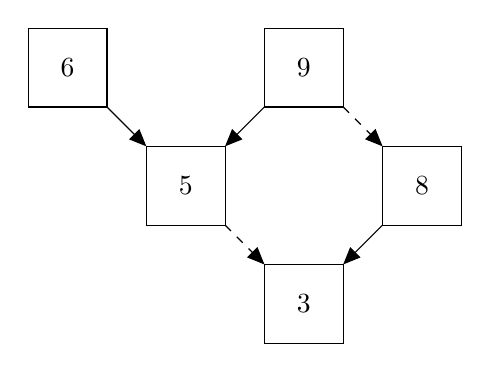
\begin{tikzpicture}[>=triangle 45]
      \draw (0,3) rectangle (1,4) node[pos=0.5]{6};
      \draw (1.5,1.5) rectangle (2.5,2.5) node[pos=0.5]{5};
      \draw (3,0) rectangle (4,1) node[pos=0.5]{3};
      \draw (3,3) rectangle (4,4) node[pos=0.5]{9};
      \draw (4.5,1.5) rectangle (5.5,2.5) node[pos=0.5]{8};
      \draw [->] (1,3) -- (1.5,2.5); % 6 -> 5
      \draw [->, dashed] (2.5,1.5) -- (3,1); % 5 -> 3
      \draw [->] (3,3) -- (2.5,2.5); % 9 -> 5
      \draw [->, dashed] (4,3) -- (4.5,2.5); % 9 -> 8
      \draw [->] (4.5,1.5) -- (4,1); % 8 -> 3
    \end{tikzpicture}
  \end{center}
  \caption{Dependencies between the chapters of TAPL}
  \label{fig:TAPL-dependencies}
\end{figure}

The formalization closely follows the structure of the book. We provide one Isabelle theory file per
chapter and mainly introduce them in the same order. The only exception is the chapter on "Nameless
Representation of Terms". In the book, it is treated as a completely separate issue from the
chapters on $\lambda$-calculus (i.e. an encoding that can be useful for an implementation). They
present it as a concrete alternative to the implicit $\alpha$-conversion they assume in their
proofs, which is nice for humans but not rigorous enough for a computer. Even though a formalization
is different from an implementation it have some similar requirements. Since we chose this nameless
representation for our formalization, we must diverge from the book and introduce this subject
before the untyped $\lambda$-calculus. Figure \ref{fig:thys-dependencies} presents the dependencies
between our Isabelle theory files.

\begin{figure}[h]
  \begin{center}
    \begin{tikzpicture}[>=triangle 45]
      \draw (0,3) rectangle (1,4) node[pos=0.5]{6};
      \draw (1.5,1.5) rectangle (2.5,2.5) node[pos=0.5]{5};
      \draw (3,0) rectangle (4,1) node[pos=0.5]{3};
      \draw (3,3) rectangle (4,4) node[pos=0.5]{9};
      \draw (4.5,1.5) rectangle (5.5,2.5) node[pos=0.5]{8};
      \draw [->, dotted] (1.5,2.5) -- (1,3); % 5 -> 6
      \draw [->, dashed] (2.5,1.5) -- (3,1); % 5 -> 3
      \draw [->] (3,3) -- (2.5,2.5); % 9 -> 5
      \draw [->, dashed] (4,3) -- (4.5,2.5); % 9 -> 8
      \draw [->, dotted] (4.5,1.5) -- (4,1); % 8 -> 3
    \end{tikzpicture}
  \end{center}
  \caption{Dependencies between the theory files}
  \label{fig:thys-dependencies}
\end{figure}

It was possible to directly base the typed arithmetic expressions on untyped arithmetic expression
by importing the theory and reusing its definition. This is represented as a dotted arrow in figure
\ref{fig:thys-dependencies}. This reuse is possible because, for this language, types are external
to the representation of terms. By contrast, for the typed $\lambda$-calculus, we need to alter the
representation of terms to add the typing annotation on abstraction variables, thus preventing the
reuse of the untyped $\lambda$-calculus theory.


% sane default for proof documents
\parindent 0pt\parskip 0.5ex

\part{Untyped Systems}
\input{Untyped_Arithmetic_Expressions.tex}
\input{Nameless_Representation_Of_Terms.tex}
\input{Untyped_Lambda_Calculus.tex}

\part{Typed Systems}
\input{Typed_Arithmetic_Expressions.tex}
\input{Typed_Lambda_Calculus.tex}

\part{Conclusion}
\section{Conclusion}

We formalized a number of languages present in \emph{Types and Programming Languages} with the
Isabelle/HOL interactive theorem prover. We started with a simple arithmetic language of booleans
and natural numbers. We continued with the nameless representation of terms for the
$\lambda$-calculus, which we used as a basis for the pure untyped $\lambda$-calculus. For those
languages, we proved the determinacy of evaluation, the relation between values and normal form, the
uniqueness of normal form and the termination, or non-termination, of evaluation.

We then revisited both languages and augment them with type systems. We proved the uniqueness of
types and the safety of the languages through the progress and preservation theorems. We also
demonstrated that the addition of types did not changed the semantic of the $\lambda$-calculus by
proving that types can be erase without affecting the evaluation of terms.

The formalization process can be separate in three main activies: defining the primitives,
formulating the theorems and finally the proving per se. In retrospective, the first and second
activities were the more important and difficult. Once the right abstractions and the correct
formulations for theorems were found, the proofs were usually fairly simple. On the contrary, a
wrong abstraction or hypothesis have led use to theorems very difficult to prove, or even properties
that ended not being theorems at all.

In this report, we focused our attention on the definitions on how theorems were expressed,
highlighting the differences with the book. The complete Isabelle/HOL theories provided along this
report contain more examples, exercices and less important theorems.


% optional bibliography
%\bibliographystyle{abbrv}
%\bibliography{root}

\end{document}

%%% Local Variables:
%%% mode: latex
%%% TeX-master: t
%%% End:
